\documentclass[1p]{elsarticle_modified}
%\bibliographystyle{elsarticle-num}

%\usepackage[colorlinks]{hyperref}
%\usepackage{abbrmath_seonhwa} %\Abb, \Ascr, \Acal ,\Abf, \Afrak
\usepackage{amsfonts}
\usepackage{amssymb}
\usepackage{amsmath}
\usepackage{amsthm}
\usepackage{scalefnt}
\usepackage{amsbsy}
\usepackage{kotex}
\usepackage{caption}
\usepackage{subfig}
\usepackage{color}
\usepackage{graphicx}
\usepackage{xcolor} %% white, black, red, green, blue, cyan, magenta, yellow
\usepackage{float}
\usepackage{setspace}
\usepackage{hyperref}

\usepackage{tikz}
\usetikzlibrary{arrows}

\usepackage{multirow}
\usepackage{array} % fixed length table
\usepackage{hhline}

%%%%%%%%%%%%%%%%%%%%%
\makeatletter
\renewcommand*\env@matrix[1][\arraystretch]{%
	\edef\arraystretch{#1}%
	\hskip -\arraycolsep
	\let\@ifnextchar\new@ifnextchar
	\array{*\c@MaxMatrixCols c}}
\makeatother %https://tex.stackexchange.com/questions/14071/how-can-i-increase-the-line-spacing-in-a-matrix
%%%%%%%%%%%%%%%

\usepackage[normalem]{ulem}

\newcommand{\msout}[1]{\ifmmode\text{\sout{\ensuremath{#1}}}\else\sout{#1}\fi}
%SOURCE: \msout is \stkout macro in https://tex.stackexchange.com/questions/20609/strikeout-in-math-mode

\newcommand{\cancel}[1]{
	\ifmmode
	{\color{red}\msout{#1}}
	\else
	{\color{red}\sout{#1}}
	\fi
}

\newcommand{\add}[1]{
	{\color{blue}\uwave{#1}}
}

\newcommand{\replace}[2]{
	\ifmmode
	{\color{red}\msout{#1}}{\color{blue}\uwave{#2}}
	\else
	{\color{red}\sout{#1}}{\color{blue}\uwave{#2}}
	\fi
}

\newcommand{\Sol}{\mathcal{S}} %segment
\newcommand{\D}{D} %diagram
\newcommand{\A}{\mathcal{A}} %arc


%%%%%%%%%%%%%%%%%%%%%%%%%%%%%5 test

\def\sl{\operatorname{\textup{SL}}(2,\Cbb)}
\def\psl{\operatorname{\textup{PSL}}(2,\Cbb)}
\def\quan{\mkern 1mu \triangleright \mkern 1mu}

\theoremstyle{definition}
\newtheorem{thm}{Theorem}[section]
\newtheorem{prop}[thm]{Proposition}
\newtheorem{lem}[thm]{Lemma}
\newtheorem{ques}[thm]{Question}
\newtheorem{cor}[thm]{Corollary}
\newtheorem{defn}[thm]{Definition}
\newtheorem{exam}[thm]{Example}
\newtheorem{rmk}[thm]{Remark}
\newtheorem{alg}[thm]{Algorithm}

\newcommand{\I}{\sqrt{-1}}
\begin{document}

%\begin{frontmatter}
%
%\title{Boundary parabolic representations of knots up to 8 crossings}
%
%%% Group authors per affiliation:
%\author{Yunhi Cho} 
%\address{Department of Mathematics, University of Seoul, Seoul, Korea}
%\ead{yhcho@uos.ac.kr}
%
%
%\author{Seonhwa Kim} %\fnref{s_kim}}
%\address{Center for Geometry and Physics, Institute for Basic Science, Pohang, 37673, Korea}
%\ead{ryeona17@ibs.re.kr}
%
%\author{Hyuk Kim}
%\address{Department of Mathematical Sciences, Seoul National University, Seoul 08826, Korea}
%\ead{hyukkim@snu.ac.kr}
%
%\author{Seokbeom Yoon}
%\address{Department of Mathematical Sciences, Seoul National University, Seoul, 08826,  Korea}
%\ead{sbyoon15@snu.ac.kr}
%
%\begin{abstract}
%We find all boundary parabolic representation of knots up to 8 crossings.
%
%\end{abstract}
%\begin{keyword}
%    \MSC[2010] 57M25 
%\end{keyword}
%
%\end{frontmatter}

%\linenumbers
%\tableofcontents
%
\newcommand\colored[1]{\textcolor{white}{\rule[-0.35ex]{0.8em}{1.4ex}}\kern-0.8em\color{red} #1}%
%\newcommand\colored[1]{\textcolor{white}{ #1}\kern-2.17ex	\textcolor{white}{ #1}\kern-1.81ex	\textcolor{white}{ #1}\kern-2.15ex\color{red}#1	}

{\Large $\underline{12a_{0648}~(K12a_{0648})}$}

\setlength{\tabcolsep}{10pt}
\renewcommand{\arraystretch}{1.6}
\vspace{1cm}\begin{tabular}{m{100pt}>{\centering\arraybackslash}m{274pt}}
\multirow{5}{120pt}{
	\centering
	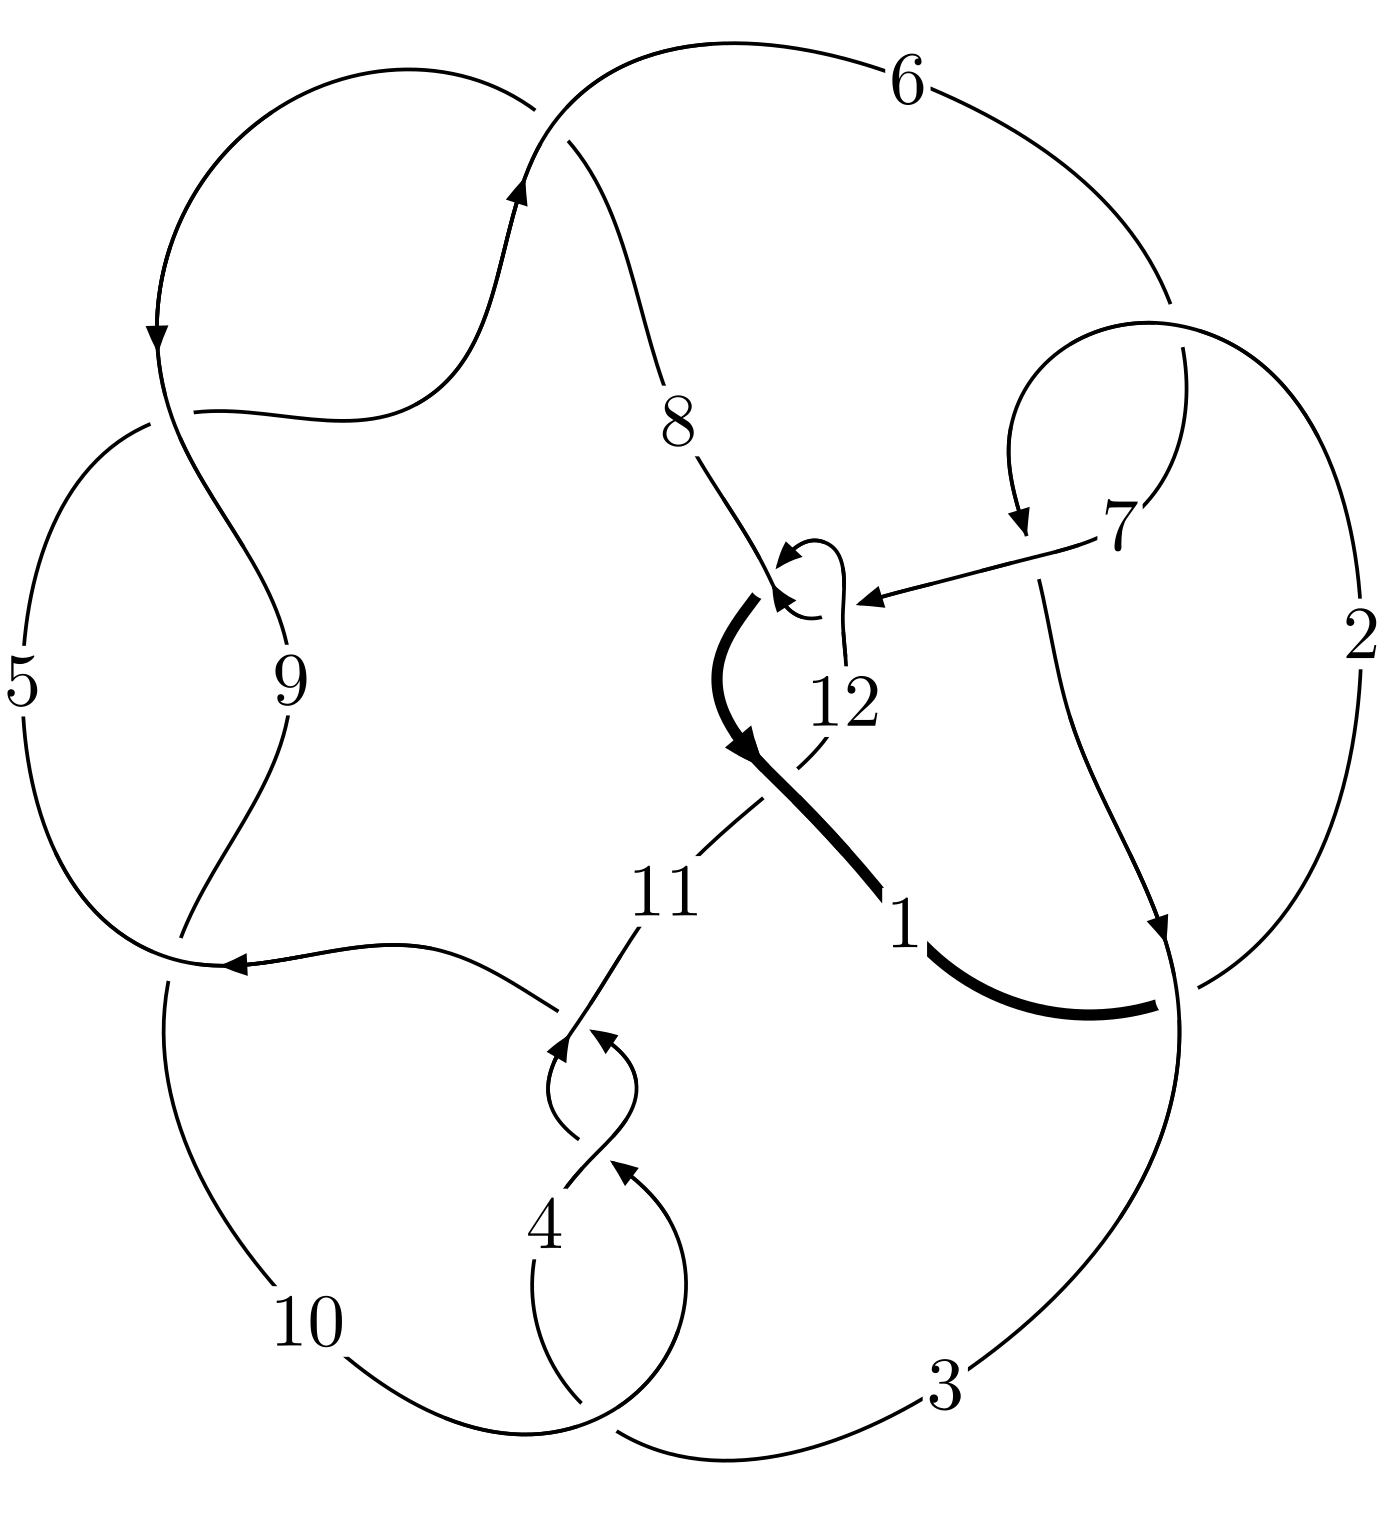
\includegraphics[width=112pt]{../../../GIT/diagram.site/Diagrams/png/1449_12a_0648.png}\\
\ \ \ A knot diagram\footnotemark}&
\allowdisplaybreaks
\textbf{Linearized knot diagam} \\
\cline{2-2}
 &
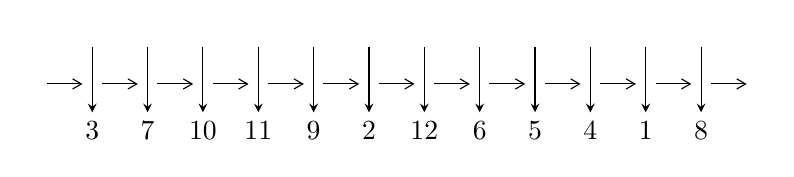
\begin{tikzpicture}[x=20pt, y=17pt]
	% nodes
	\node (C0) at (0, 0) {};
	\node (C1) at (1, 0) {};
	\node (C1U) at (1, +1) {};
	\node (C1D) at (1, -1) {3};

	\node (C2) at (2, 0) {};
	\node (C2U) at (2, +1) {};
	\node (C2D) at (2, -1) {7};

	\node (C3) at (3, 0) {};
	\node (C3U) at (3, +1) {};
	\node (C3D) at (3, -1) {10};

	\node (C4) at (4, 0) {};
	\node (C4U) at (4, +1) {};
	\node (C4D) at (4, -1) {11};

	\node (C5) at (5, 0) {};
	\node (C5U) at (5, +1) {};
	\node (C5D) at (5, -1) {9};

	\node (C6) at (6, 0) {};
	\node (C6U) at (6, +1) {};
	\node (C6D) at (6, -1) {2};

	\node (C7) at (7, 0) {};
	\node (C7U) at (7, +1) {};
	\node (C7D) at (7, -1) {12};

	\node (C8) at (8, 0) {};
	\node (C8U) at (8, +1) {};
	\node (C8D) at (8, -1) {6};

	\node (C9) at (9, 0) {};
	\node (C9U) at (9, +1) {};
	\node (C9D) at (9, -1) {5};

	\node (C10) at (10, 0) {};
	\node (C10U) at (10, +1) {};
	\node (C10D) at (10, -1) {4};

	\node (C11) at (11, 0) {};
	\node (C11U) at (11, +1) {};
	\node (C11D) at (11, -1) {1};

	\node (C12) at (12, 0) {};
	\node (C12U) at (12, +1) {};
	\node (C12D) at (12, -1) {8};
	\node (C13) at (13, 0) {};

	% arrows
	\draw[->,>={angle 60}]
	(C0) edge (C1) (C1) edge (C2) (C2) edge (C3) (C3) edge (C4) (C4) edge (C5) (C5) edge (C6) (C6) edge (C7) (C7) edge (C8) (C8) edge (C9) (C9) edge (C10) (C10) edge (C11) (C11) edge (C12) (C12) edge (C13) ;	\draw[->,>=stealth]
	(C1U) edge (C1D) (C2U) edge (C2D) (C3U) edge (C3D) (C4U) edge (C4D) (C5U) edge (C5D) (C6U) edge (C6D) (C7U) edge (C7D) (C8U) edge (C8D) (C9U) edge (C9D) (C10U) edge (C10D) (C11U) edge (C11D) (C12U) edge (C12D) ;
	\end{tikzpicture} \\
\hhline{~~} \\& 
\textbf{Solving Sequence} \\ \cline{2-2} 
 &
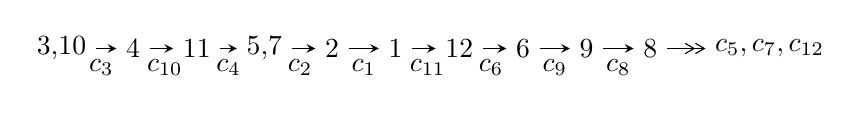
\begin{tikzpicture}[x=23pt, y=7pt]
	% node
	\node (A0) at (-1/8, 0) {3,10};
	\node (A1) at (1, 0) {4};
	\node (A2) at (2, 0) {11};
	\node (A3) at (49/16, 0) {5,7};
	\node (A4) at (33/8, 0) {2};
	\node (A5) at (41/8, 0) {1};
	\node (A6) at (49/8, 0) {12};
	\node (A7) at (57/8, 0) {6};
	\node (A8) at (65/8, 0) {9};
	\node (A9) at (73/8, 0) {8};
	\node (C1) at (1/2, -1) {$c_{3}$};
	\node (C2) at (3/2, -1) {$c_{10}$};
	\node (C3) at (5/2, -1) {$c_{4}$};
	\node (C4) at (29/8, -1) {$c_{2}$};
	\node (C5) at (37/8, -1) {$c_{1}$};
	\node (C6) at (45/8, -1) {$c_{11}$};
	\node (C7) at (53/8, -1) {$c_{6}$};
	\node (C8) at (61/8, -1) {$c_{9}$};
	\node (C9) at (69/8, -1) {$c_{8}$};
	\node (A10) at (11, 0) {$c_{5},c_{7},c_{12}$};

	% edge
	\draw[->,>=stealth]	
	(A0) edge (A1) (A1) edge (A2) (A2) edge (A3) (A3) edge (A4) (A4) edge (A5) (A5) edge (A6) (A6) edge (A7) (A7) edge (A8) (A8) edge (A9) ;
	\draw[->>,>={angle 60}]	
	(A9) edge (A10);
\end{tikzpicture} \\ 

\end{tabular} \\

\footnotetext{
The image of knot diagram is generated by the software ``\textbf{Draw programme}" developed by Andrew Bartholomew(\url{http://www.layer8.co.uk/maths/draw/index.htm\#Running-draw}), where we modified some parts for our purpose(\url{https://github.com/CATsTAILs/LinksPainter}).
}\phantom \\ \newline 
\centering \textbf{Ideals for irreducible components\footnotemark of $X_{\text{par}}$} 
 
\begin{align*}
I^u_{1}&=\langle 
- u^{33}+u^{32}+\cdots+b-1,\;u^{33}- u^{32}+\cdots+2 a+u,\;u^{34}-3 u^{33}+\cdots+7 u^2-2\rangle \\
I^u_{2}&=\langle 
40 u^{23} a+70 u^{23}+\cdots+34 a+57,\;2 u^{23} a+u^{23}+\cdots+a^2+2,\;u^{24}+u^{23}+\cdots+2 u^2+1\rangle \\
I^u_{3}&=\langle 
b-1,\;-2 u^3+3 u^2+3 a+3 u-6,\;u^4-3 u^2+3\rangle \\
I^u_{4}&=\langle 
b+1,\;u^2+a- u,\;u^4- u^2-1\rangle \\
\\
I^v_{1}&=\langle 
a,\;b-1,\;v+1\rangle \\
\end{align*}
\raggedright * 5 irreducible components of $\dim_{\mathbb{C}}=0$, with total 91 representations.\\
\footnotetext{All coefficients of polynomials are rational numbers. But the coefficients are sometimes approximated in decimal forms when there is not enough margin.}
\newpage
\renewcommand{\arraystretch}{1}
\centering \section*{I. $I^u_{1}= \langle - u^{33}+u^{32}+\cdots+b-1,\;u^{33}- u^{32}+\cdots+2 a+u,\;u^{34}-3 u^{33}+\cdots+7 u^2-2 \rangle$}
\flushleft \textbf{(i) Arc colorings}\\
\begin{tabular}{m{7pt} m{180pt} m{7pt} m{180pt} }
\flushright $a_{3}=$&$\begin{pmatrix}1\\0\end{pmatrix}$ \\
\flushright $a_{10}=$&$\begin{pmatrix}0\\u\end{pmatrix}$ \\
\flushright $a_{4}=$&$\begin{pmatrix}1\\u^2\end{pmatrix}$ \\
\flushright $a_{11}=$&$\begin{pmatrix}- u\\- u^3+u\end{pmatrix}$ \\
\flushright $a_{5}=$&$\begin{pmatrix}- u^2+1\\- u^4+2 u^2\end{pmatrix}$ \\
\flushright $a_{7}=$&$\begin{pmatrix}-\frac{1}{2} u^{33}+\frac{1}{2} u^{32}+\cdots+2 u^2-\frac{1}{2} u\\u^{33}- u^{32}+\cdots+u+1\end{pmatrix}$ \\
\flushright $a_{2}=$&$\begin{pmatrix}\frac{7}{2} u^{33}-\frac{13}{2} u^{32}+\cdots+\frac{7}{2} u+6\\u^{33}-2 u^{32}+\cdots+2 u+1\end{pmatrix}$ \\
\flushright $a_{1}=$&$\begin{pmatrix}\frac{9}{2} u^{33}-\frac{17}{2} u^{32}+\cdots+\frac{11}{2} u+7\\u^{33}-2 u^{32}+\cdots+2 u+1\end{pmatrix}$ \\
\flushright $a_{12}=$&$\begin{pmatrix}\frac{7}{2} u^{33}-\frac{13}{2} u^{32}+\cdots+\frac{5}{2} u+5\\u^{33}-2 u^{32}+\cdots+3 u+1\end{pmatrix}$ \\
\flushright $a_{6}=$&$\begin{pmatrix}- u^8+3 u^6-3 u^4+1\\- u^{10}+4 u^8-5 u^6+3 u^2\end{pmatrix}$ \\
\flushright $a_{9}=$&$\begin{pmatrix}u^5-2 u^3+u\\u^7-3 u^5+2 u^3+u\end{pmatrix}$ \\
\flushright $a_{8}=$&$\begin{pmatrix}u^{11}-4 u^9+6 u^7-2 u^5-3 u^3+2 u\\u^{13}-5 u^{11}+9 u^9-4 u^7-6 u^5+5 u^3+u\end{pmatrix}$\\&\end{tabular}
\flushleft \textbf{(ii) Obstruction class $= -1$}\\~\\
\flushleft \textbf{(iii) Cusp Shapes $= 16 u^{33}-30 u^{32}-176 u^{31}+310 u^{30}+906 u^{29}-1386 u^{28}-2824 u^{27}+3246 u^{26}+5702 u^{25}-3296 u^{24}-7040 u^{23}-2332 u^{22}+3058 u^{21}+10882 u^{20}+6024 u^{19}-10740 u^{18}-12104 u^{17}-2002 u^{16}+6950 u^{15}+11788 u^{14}+4152 u^{13}-6006 u^{12}-7292 u^{11}-3698 u^{10}+1314 u^9+3622 u^8+2284 u^7+444 u^6-662 u^5-734 u^4-368 u^3-88 u^2+8 u+12$}\\~\\
\newpage\renewcommand{\arraystretch}{1}
\flushleft \textbf{(iv) u-Polynomials at the component}\newline \\
\begin{tabular}{m{50pt}|m{274pt}}
Crossings & \hspace{64pt}u-Polynomials at each crossing \\
\hline $$\begin{aligned}c_{1},c_{11}\end{aligned}$$&$\begin{aligned}
&u^{34}+13 u^{33}+\cdots+18 u+1
\end{aligned}$\\
\hline $$\begin{aligned}c_{2},c_{6},c_{7}\\c_{12}\end{aligned}$$&$\begin{aligned}
&u^{34}- u^{33}+\cdots-2 u-1
\end{aligned}$\\
\hline $$\begin{aligned}c_{3},c_{4},c_{10}\end{aligned}$$&$\begin{aligned}
&u^{34}+3 u^{33}+\cdots+7 u^2-2
\end{aligned}$\\
\hline $$\begin{aligned}c_{5},c_{8},c_{9}\end{aligned}$$&$\begin{aligned}
&u^{34}-9 u^{33}+\cdots-104 u+14
\end{aligned}$\\
\hline
\end{tabular}\\~\\
\newpage\renewcommand{\arraystretch}{1}
\flushleft \textbf{(v) Riley Polynomials at the component}\newline \\
\begin{tabular}{m{50pt}|m{274pt}}
Crossings & \hspace{64pt}Riley Polynomials at each crossing \\
\hline $$\begin{aligned}c_{1},c_{11}\end{aligned}$$&$\begin{aligned}
&y^{34}+27 y^{33}+\cdots-46 y+1
\end{aligned}$\\
\hline $$\begin{aligned}c_{2},c_{6},c_{7}\\c_{12}\end{aligned}$$&$\begin{aligned}
&y^{34}-13 y^{33}+\cdots-18 y+1
\end{aligned}$\\
\hline $$\begin{aligned}c_{3},c_{4},c_{10}\end{aligned}$$&$\begin{aligned}
&y^{34}-27 y^{33}+\cdots-28 y+4
\end{aligned}$\\
\hline $$\begin{aligned}c_{5},c_{8},c_{9}\end{aligned}$$&$\begin{aligned}
&y^{34}+33 y^{33}+\cdots-540 y+196
\end{aligned}$\\
\hline
\end{tabular}\\~\\
\newpage\flushleft \textbf{(vi) Complex Volumes and Cusp Shapes}
$$\begin{array}{c|c|c}  
\text{Solutions to }I^u_{1}& \I (\text{vol} + \sqrt{-1}CS) & \text{Cusp shape}\\
 \hline 
\begin{aligned}
u &= -1.013520 + 0.242521 I \\
a &= \phantom{-}0.355644 + 1.026690 I \\
b &= \phantom{-}0.890943 - 0.630816 I\end{aligned}
 & -0.60916 + 4.94810 I & -11.40571 - 6.58430 I \\ \hline\begin{aligned}
u &= -1.013520 - 0.242521 I \\
a &= \phantom{-}0.355644 - 1.026690 I \\
b &= \phantom{-}0.890943 + 0.630816 I\end{aligned}
 & -0.60916 - 4.94810 I & -11.40571 + 6.58430 I \\ \hline\begin{aligned}
u &= -0.019993 + 0.886536 I \\
a &= -0.99279 - 1.72000 I \\
b &= \phantom{-}0.620427 + 0.888173 I\end{aligned}
 & \phantom{-}10.23300 - 0.57498 I & -4.93221 + 2.01552 I \\ \hline\begin{aligned}
u &= -0.019993 - 0.886536 I \\
a &= -0.99279 + 1.72000 I \\
b &= \phantom{-}0.620427 - 0.888173 I\end{aligned}
 & \phantom{-}10.23300 + 0.57498 I & -4.93221 - 2.01552 I \\ \hline\begin{aligned}
u &= -0.068695 + 0.879558 I \\
a &= -0.61168 + 2.14998 I \\
b &= \phantom{-}1.162480 - 0.677594 I\end{aligned}
 & \phantom{-}6.70898 + 11.31000 I & -9.03751 - 7.13336 I \\ \hline\begin{aligned}
u &= -0.068695 - 0.879558 I \\
a &= -0.61168 - 2.14998 I \\
b &= \phantom{-}1.162480 + 0.677594 I\end{aligned}
 & \phantom{-}6.70898 - 11.31000 I & -9.03751 + 7.13336 I \\ \hline\begin{aligned}
u &= \phantom{-}1.207750 + 0.187996 I \\
a &= -0.308967 + 0.091247 I \\
b &= \phantom{-}0.324451 - 0.579872 I\end{aligned}
 & -1.55132 - 1.46622 I & -9.64070 + 0.44653 I \\ \hline\begin{aligned}
u &= \phantom{-}1.207750 - 0.187996 I \\
a &= -0.308967 - 0.091247 I \\
b &= \phantom{-}0.324451 + 0.579872 I\end{aligned}
 & -1.55132 + 1.46622 I & -9.64070 - 0.44653 I \\ \hline\begin{aligned}
u &= -1.211280 + 0.430207 I \\
a &= \phantom{-}0.282844 + 0.666214 I \\
b &= -1.145270 - 0.686416 I\end{aligned}
 & \phantom{-}3.19057 - 6.62584 I & -12.00000 + 3.79448 I \\ \hline\begin{aligned}
u &= -1.211280 - 0.430207 I \\
a &= \phantom{-}0.282844 - 0.666214 I \\
b &= -1.145270 + 0.686416 I\end{aligned}
 & \phantom{-}3.19057 + 6.62584 I & -12.00000 - 3.79448 I\\
 \hline 
 \end{array}$$\newpage$$\begin{array}{c|c|c}  
\text{Solutions to }I^u_{1}& \I (\text{vol} + \sqrt{-1}CS) & \text{Cusp shape}\\
 \hline 
\begin{aligned}
u &= -0.086828 + 0.686695 I \\
a &= \phantom{-}0.675634 + 0.571144 I \\
b &= -0.750792 - 0.491169 I\end{aligned}
 & \phantom{-}2.05021 - 1.49541 I & -7.38318 + 3.42302 I \\ \hline\begin{aligned}
u &= -0.086828 - 0.686695 I \\
a &= \phantom{-}0.675634 - 0.571144 I \\
b &= -0.750792 + 0.491169 I\end{aligned}
 & \phantom{-}2.05021 + 1.49541 I & -7.38318 - 3.42302 I \\ \hline\begin{aligned}
u &= -1.31718\phantom{ +0.000000I} \\
a &= -1.28254\phantom{ +0.000000I} \\
b &= -0.594449\phantom{ +0.000000I}\end{aligned}
 & -5.52603\phantom{ +0.000000I} & -16.4440\phantom{ +0.000000I} \\ \hline\begin{aligned}
u &= -1.281510 + 0.305200 I \\
a &= \phantom{-}0.845662 + 0.733598 I \\
b &= \phantom{-}0.682471 - 0.253099 I\end{aligned}
 & -1.94338 + 5.09853 I & -12.0000 - 8.2909 I \\ \hline\begin{aligned}
u &= -1.281510 - 0.305200 I \\
a &= \phantom{-}0.845662 - 0.733598 I \\
b &= \phantom{-}0.682471 + 0.253099 I\end{aligned}
 & -1.94338 - 5.09853 I & -12.0000 + 8.2909 I \\ \hline\begin{aligned}
u &= -1.260670 + 0.425063 I \\
a &= -0.21847 - 1.46519 I \\
b &= -0.653525 + 0.878185 I\end{aligned}
 & \phantom{-}6.38980 + 5.26542 I & -8.46055 - 5.30635 I \\ \hline\begin{aligned}
u &= -1.260670 - 0.425063 I \\
a &= -0.21847 + 1.46519 I \\
b &= -0.653525 - 0.878185 I\end{aligned}
 & \phantom{-}6.38980 - 5.26542 I & -8.46055 + 5.30635 I \\ \hline\begin{aligned}
u &= -0.007042 + 0.669070 I \\
a &= \phantom{-}0.407696 + 0.768480 I \\
b &= -0.636123 - 0.421028 I\end{aligned}
 & \phantom{-}2.05008 - 1.46908 I & -6.49670 + 4.60453 I \\ \hline\begin{aligned}
u &= -0.007042 - 0.669070 I \\
a &= \phantom{-}0.407696 - 0.768480 I \\
b &= -0.636123 + 0.421028 I\end{aligned}
 & \phantom{-}2.05008 + 1.46908 I & -6.49670 - 4.60453 I \\ \hline\begin{aligned}
u &= -0.584426 + 0.322111 I \\
a &= \phantom{-}0.0940661 - 0.0123771 I \\
b &= \phantom{-}0.998997 + 0.590488 I\end{aligned}
 & -1.17138 - 4.75212 I & -13.33145 + 3.31691 I\\
 \hline 
 \end{array}$$\newpage$$\begin{array}{c|c|c}  
\text{Solutions to }I^u_{1}& \I (\text{vol} + \sqrt{-1}CS) & \text{Cusp shape}\\
 \hline 
\begin{aligned}
u &= -0.584426 - 0.322111 I \\
a &= \phantom{-}0.0940661 + 0.0123771 I \\
b &= \phantom{-}0.998997 - 0.590488 I\end{aligned}
 & -1.17138 + 4.75212 I & -13.33145 - 3.31691 I \\ \hline\begin{aligned}
u &= -0.331538 + 0.561990 I \\
a &= -0.42743 - 2.05569 I \\
b &= -1.071630 + 0.613723 I\end{aligned}
 & -0.24987 + 8.13095 I & -11.3800 - 9.4182 I \\ \hline\begin{aligned}
u &= -0.331538 - 0.561990 I \\
a &= -0.42743 + 2.05569 I \\
b &= -1.071630 - 0.613723 I\end{aligned}
 & -0.24987 - 8.13095 I & -11.3800 + 9.4182 I \\ \hline\begin{aligned}
u &= \phantom{-}1.312450 + 0.320860 I \\
a &= \phantom{-}0.246500 - 0.701851 I \\
b &= \phantom{-}0.854983 - 0.402484 I\end{aligned}
 & -2.29444 - 2.26511 I & -13.59499 - 1.93125 I \\ \hline\begin{aligned}
u &= \phantom{-}1.312450 - 0.320860 I \\
a &= \phantom{-}0.246500 + 0.701851 I \\
b &= \phantom{-}0.854983 + 0.402484 I\end{aligned}
 & -2.29444 + 2.26511 I & -13.59499 + 1.93125 I \\ \hline\begin{aligned}
u &= \phantom{-}1.292790 + 0.415380 I \\
a &= \phantom{-}1.050280 - 0.475483 I \\
b &= -0.587435 + 0.891176 I\end{aligned}
 & \phantom{-}6.14677 - 4.08463 I & -8.53251 + 0. I\phantom{ +0.000000I} \\ \hline\begin{aligned}
u &= \phantom{-}1.292790 - 0.415380 I \\
a &= \phantom{-}1.050280 + 0.475483 I \\
b &= -0.587435 - 0.891176 I\end{aligned}
 & \phantom{-}6.14677 + 4.08463 I & -8.53251 + 0. I\phantom{ +0.000000I} \\ \hline\begin{aligned}
u &= \phantom{-}1.365780 + 0.061291 I \\
a &= -1.52752 + 0.49479 I \\
b &= -1.016200 + 0.501862 I\end{aligned}
 & -7.06900 + 3.73055 I & -18.8014 - 4.5700 I \\ \hline\begin{aligned}
u &= \phantom{-}1.365780 - 0.061291 I \\
a &= -1.52752 - 0.49479 I \\
b &= -1.016200 - 0.501862 I\end{aligned}
 & -7.06900 - 3.73055 I & -18.8014 + 4.5700 I \\ \hline\begin{aligned}
u &= \phantom{-}1.356100 + 0.180668 I \\
a &= \phantom{-}1.87588 - 1.22676 I \\
b &= \phantom{-}1.113880 + 0.583314 I\end{aligned}
 & -5.54762 - 10.69250 I & -17.2417 + 9.2859 I\\
 \hline 
 \end{array}$$\newpage$$\begin{array}{c|c|c}  
\text{Solutions to }I^u_{1}& \I (\text{vol} + \sqrt{-1}CS) & \text{Cusp shape}\\
 \hline 
\begin{aligned}
u &= \phantom{-}1.356100 - 0.180668 I \\
a &= \phantom{-}1.87588 + 1.22676 I \\
b &= \phantom{-}1.113880 - 0.583314 I\end{aligned}
 & -5.54762 + 10.69250 I & -17.2417 - 9.2859 I \\ \hline\begin{aligned}
u &= \phantom{-}1.325120 + 0.401209 I \\
a &= -0.95387 + 2.20135 I \\
b &= -1.173850 - 0.667200 I\end{aligned}
 & \phantom{-}2.3480 - 15.9016 I & -12.0000 + 9.6149 I \\ \hline\begin{aligned}
u &= \phantom{-}1.325120 - 0.401209 I \\
a &= -0.95387 - 2.20135 I \\
b &= -1.173850 + 0.667200 I\end{aligned}
 & \phantom{-}2.3480 + 15.9016 I & -12.0000 - 9.6149 I \\ \hline\begin{aligned}
u &= \phantom{-}0.328225\phantom{ +0.000000I} \\
a &= \phantom{-}0.695567\phantom{ +0.000000I} \\
b &= \phantom{-}0.366829\phantom{ +0.000000I}\end{aligned}
 & -0.582542\phantom{ +0.000000I} & -16.9630\phantom{ +0.000000I}\\
 \hline 
 \end{array}$$\newpage\newpage\renewcommand{\arraystretch}{1}
\centering \section*{II. $I^u_{2}= \langle 40 u^{23} a+70 u^{23}+\cdots+34 a+57,\;2 u^{23} a+u^{23}+\cdots+a^2+2,\;u^{24}+u^{23}+\cdots+2 u^2+1 \rangle$}
\flushleft \textbf{(i) Arc colorings}\\
\begin{tabular}{m{7pt} m{180pt} m{7pt} m{180pt} }
\flushright $a_{3}=$&$\begin{pmatrix}1\\0\end{pmatrix}$ \\
\flushright $a_{10}=$&$\begin{pmatrix}0\\u\end{pmatrix}$ \\
\flushright $a_{4}=$&$\begin{pmatrix}1\\u^2\end{pmatrix}$ \\
\flushright $a_{11}=$&$\begin{pmatrix}- u\\- u^3+u\end{pmatrix}$ \\
\flushright $a_{5}=$&$\begin{pmatrix}- u^2+1\\- u^4+2 u^2\end{pmatrix}$ \\
\flushright $a_{7}=$&$\begin{pmatrix}a\\-20 u^{23} a-35 u^{23}+\cdots-17 a-\frac{57}{2}\end{pmatrix}$ \\
\flushright $a_{2}=$&$\begin{pmatrix}-35 u^{23} a-\frac{121}{2} u^{23}+\cdots-\frac{57}{2} a-50\\-\frac{23}{2} u^{23} a-21 u^{23}+\cdots-9 a-18\end{pmatrix}$ \\
\flushright $a_{1}=$&$\begin{pmatrix}-\frac{93}{2} u^{23} a-\frac{163}{2} u^{23}+\cdots-\frac{75}{2} a-68\\-\frac{23}{2} u^{23} a-21 u^{23}+\cdots-9 a-18\end{pmatrix}$ \\
\flushright $a_{12}=$&$\begin{pmatrix}35 u^{23} a+\frac{121}{2} u^{23}+\cdots+\frac{57}{2} a+51\\1\end{pmatrix}$ \\
\flushright $a_{6}=$&$\begin{pmatrix}- u^8+3 u^6-3 u^4+1\\- u^{10}+4 u^8-5 u^6+3 u^2\end{pmatrix}$ \\
\flushright $a_{9}=$&$\begin{pmatrix}u^5-2 u^3+u\\u^7-3 u^5+2 u^3+u\end{pmatrix}$ \\
\flushright $a_{8}=$&$\begin{pmatrix}u^{11}-4 u^9+6 u^7-2 u^5-3 u^3+2 u\\u^{13}-5 u^{11}+9 u^9-4 u^7-6 u^5+5 u^3+u\end{pmatrix}$\\&\end{tabular}
\flushleft \textbf{(ii) Obstruction class $= -1$}\\~\\
\flushleft \textbf{(iii) Cusp Shapes $= 4 u^{21}-32 u^{19}+4 u^{18}+108 u^{17}-28 u^{16}-180 u^{15}+80 u^{14}+104 u^{13}-104 u^{12}+120 u^{11}+24 u^{10}-216 u^9+88 u^8+56 u^7-76 u^6+80 u^5-12 u^4-36 u^3+24 u^2-8 u-10$}\\~\\
\newpage\renewcommand{\arraystretch}{1}
\flushleft \textbf{(iv) u-Polynomials at the component}\newline \\
\begin{tabular}{m{50pt}|m{274pt}}
Crossings & \hspace{64pt}u-Polynomials at each crossing \\
\hline $$\begin{aligned}c_{1},c_{11}\end{aligned}$$&$\begin{aligned}
&u^{48}+25 u^{47}+\cdots+1100 u+49
\end{aligned}$\\
\hline $$\begin{aligned}c_{2},c_{6},c_{7}\\c_{12}\end{aligned}$$&$\begin{aligned}
&u^{48}- u^{47}+\cdots+20 u-7
\end{aligned}$\\
\hline $$\begin{aligned}c_{3},c_{4},c_{10}\end{aligned}$$&$\begin{aligned}
&(u^{24}- u^{23}+\cdots+2 u^2+1)^{2}
\end{aligned}$\\
\hline $$\begin{aligned}c_{5},c_{8},c_{9}\end{aligned}$$&$\begin{aligned}
&(u^{24}+3 u^{23}+\cdots+8 u+1)^{2}
\end{aligned}$\\
\hline
\end{tabular}\\~\\
\newpage\renewcommand{\arraystretch}{1}
\flushleft \textbf{(v) Riley Polynomials at the component}\newline \\
\begin{tabular}{m{50pt}|m{274pt}}
Crossings & \hspace{64pt}Riley Polynomials at each crossing \\
\hline $$\begin{aligned}c_{1},c_{11}\end{aligned}$$&$\begin{aligned}
&y^{48}-5 y^{47}+\cdots-196288 y+2401
\end{aligned}$\\
\hline $$\begin{aligned}c_{2},c_{6},c_{7}\\c_{12}\end{aligned}$$&$\begin{aligned}
&y^{48}-25 y^{47}+\cdots-1100 y+49
\end{aligned}$\\
\hline $$\begin{aligned}c_{3},c_{4},c_{10}\end{aligned}$$&$\begin{aligned}
&(y^{24}-19 y^{23}+\cdots+4 y+1)^{2}
\end{aligned}$\\
\hline $$\begin{aligned}c_{5},c_{8},c_{9}\end{aligned}$$&$\begin{aligned}
&(y^{24}+25 y^{23}+\cdots-20 y+1)^{2}
\end{aligned}$\\
\hline
\end{tabular}\\~\\
\newpage\flushleft \textbf{(vi) Complex Volumes and Cusp Shapes}
$$\begin{array}{c|c|c}  
\text{Solutions to }I^u_{2}& \I (\text{vol} + \sqrt{-1}CS) & \text{Cusp shape}\\
 \hline 
\begin{aligned}
u &= \phantom{-}0.047552 + 0.882738 I \\
a &= -0.93385 + 1.58747 I \\
b &= \phantom{-}0.435071 - 0.953033 I\end{aligned}
 & \phantom{-}8.92830 - 5.35992 I & -6.31714 + 3.17670 I \\ \hline\begin{aligned}
u &= \phantom{-}0.047552 + 0.882738 I \\
a &= -0.77910 - 2.11672 I \\
b &= \phantom{-}1.047250 + 0.722390 I\end{aligned}
 & \phantom{-}8.92830 - 5.35992 I & -6.31714 + 3.17670 I \\ \hline\begin{aligned}
u &= \phantom{-}0.047552 - 0.882738 I \\
a &= -0.93385 - 1.58747 I \\
b &= \phantom{-}0.435071 + 0.953033 I\end{aligned}
 & \phantom{-}8.92830 + 5.35992 I & -6.31714 - 3.17670 I \\ \hline\begin{aligned}
u &= \phantom{-}0.047552 - 0.882738 I \\
a &= -0.77910 + 2.11672 I \\
b &= \phantom{-}1.047250 - 0.722390 I\end{aligned}
 & \phantom{-}8.92830 + 5.35992 I & -6.31714 - 3.17670 I \\ \hline\begin{aligned}
u &= -0.023946 + 0.850260 I \\
a &= \phantom{-}0.854901 + 0.065619 I \\
b &= -1.327570 - 0.116085 I\end{aligned}
 & \phantom{-}2.61833 + 2.14805 I & -9.50752 - 3.24690 I \\ \hline\begin{aligned}
u &= -0.023946 + 0.850260 I \\
a &= -1.26227 + 2.30944 I \\
b &= \phantom{-}0.859183 - 0.533480 I\end{aligned}
 & \phantom{-}2.61833 + 2.14805 I & -9.50752 - 3.24690 I \\ \hline\begin{aligned}
u &= -0.023946 - 0.850260 I \\
a &= \phantom{-}0.854901 - 0.065619 I \\
b &= -1.327570 + 0.116085 I\end{aligned}
 & \phantom{-}2.61833 - 2.14805 I & -9.50752 + 3.24690 I \\ \hline\begin{aligned}
u &= -0.023946 - 0.850260 I \\
a &= -1.26227 - 2.30944 I \\
b &= \phantom{-}0.859183 + 0.533480 I\end{aligned}
 & \phantom{-}2.61833 - 2.14805 I & -9.50752 + 3.24690 I \\ \hline\begin{aligned}
u &= \phantom{-}0.832524\phantom{ +0.000000I} \\
a &= \phantom{-}0.131221 + 0.555408 I \\
b &= \phantom{-}0.682430 - 0.630183 I\end{aligned}
 & -0.0807297\phantom{ +0.000000I} & -10.4750\phantom{ +0.000000I} \\ \hline\begin{aligned}
u &= \phantom{-}0.832524\phantom{ +0.000000I} \\
a &= \phantom{-}0.131221 - 0.555408 I \\
b &= \phantom{-}0.682430 + 0.630183 I\end{aligned}
 & -0.0807297\phantom{ +0.000000I} & -10.4750\phantom{ +0.000000I}\\
 \hline 
 \end{array}$$\newpage$$\begin{array}{c|c|c}  
\text{Solutions to }I^u_{2}& \I (\text{vol} + \sqrt{-1}CS) & \text{Cusp shape}\\
 \hline 
\begin{aligned}
u &= -1.20293\phantom{ +0.000000I} \\
a &= -1.73587\phantom{ +0.000000I} \\
b &= -1.15462\phantom{ +0.000000I}\end{aligned}
 & -5.82330\phantom{ +0.000000I} & -13.8910\phantom{ +0.000000I} \\ \hline\begin{aligned}
u &= -1.20293\phantom{ +0.000000I} \\
a &= -1.78357\phantom{ +0.000000I} \\
b &= \phantom{-}0.588840\phantom{ +0.000000I}\end{aligned}
 & -5.82330\phantom{ +0.000000I} & -13.8910\phantom{ +0.000000I} \\ \hline\begin{aligned}
u &= \phantom{-}1.293390 + 0.128068 I \\
a &= -1.91095 + 0.30080 I \\
b &= -1.204290 + 0.245726 I\end{aligned}
 & -7.93370 - 2.66216 I & -20.0752 + 4.8307 I \\ \hline\begin{aligned}
u &= \phantom{-}1.293390 + 0.128068 I \\
a &= \phantom{-}1.66650 - 2.23253 I \\
b &= \phantom{-}1.051290 + 0.371289 I\end{aligned}
 & -7.93370 - 2.66216 I & -20.0752 + 4.8307 I \\ \hline\begin{aligned}
u &= \phantom{-}1.293390 - 0.128068 I \\
a &= -1.91095 - 0.30080 I \\
b &= -1.204290 - 0.245726 I\end{aligned}
 & -7.93370 + 2.66216 I & -20.0752 - 4.8307 I \\ \hline\begin{aligned}
u &= \phantom{-}1.293390 - 0.128068 I \\
a &= \phantom{-}1.66650 + 2.23253 I \\
b &= \phantom{-}1.051290 - 0.371289 I\end{aligned}
 & -7.93370 + 2.66216 I & -20.0752 - 4.8307 I \\ \hline\begin{aligned}
u &= \phantom{-}1.234200 + 0.427679 I \\
a &= \phantom{-}0.533072 - 0.692246 I \\
b &= -1.021630 + 0.732505 I\end{aligned}
 & \phantom{-}5.26485 + 0.67393 I & -9.45928 + 0.18139 I \\ \hline\begin{aligned}
u &= \phantom{-}1.234200 + 0.427679 I \\
a &= -0.175482 + 1.183140 I \\
b &= -0.464333 - 0.941817 I\end{aligned}
 & \phantom{-}5.26485 + 0.67393 I & -9.45928 + 0.18139 I \\ \hline\begin{aligned}
u &= \phantom{-}1.234200 - 0.427679 I \\
a &= \phantom{-}0.533072 + 0.692246 I \\
b &= -1.021630 - 0.732505 I\end{aligned}
 & \phantom{-}5.26485 - 0.67393 I & -9.45928 - 0.18139 I \\ \hline\begin{aligned}
u &= \phantom{-}1.234200 - 0.427679 I \\
a &= -0.175482 - 1.183140 I \\
b &= -0.464333 + 0.941817 I\end{aligned}
 & \phantom{-}5.26485 - 0.67393 I & -9.45928 - 0.18139 I\\
 \hline 
 \end{array}$$\newpage$$\begin{array}{c|c|c}  
\text{Solutions to }I^u_{2}& \I (\text{vol} + \sqrt{-1}CS) & \text{Cusp shape}\\
 \hline 
\begin{aligned}
u &= \phantom{-}0.691969\phantom{ +0.000000I} \\
a &= \phantom{-}0.274874 + 0.414868 I \\
b &= \phantom{-}0.670746 - 0.591354 I\end{aligned}
 & -0.0763260\phantom{ +0.000000I} & -11.1940\phantom{ +0.000000I} \\ \hline\begin{aligned}
u &= \phantom{-}0.691969\phantom{ +0.000000I} \\
a &= \phantom{-}0.274874 - 0.414868 I \\
b &= \phantom{-}0.670746 + 0.591354 I\end{aligned}
 & -0.0763260\phantom{ +0.000000I} & -11.1940\phantom{ +0.000000I} \\ \hline\begin{aligned}
u &= -1.30821\phantom{ +0.000000I} \\
a &= -1.11879\phantom{ +0.000000I} \\
b &= -0.332716\phantom{ +0.000000I}\end{aligned}
 & -5.51913\phantom{ +0.000000I} & -16.7540\phantom{ +0.000000I} \\ \hline\begin{aligned}
u &= -1.30821\phantom{ +0.000000I} \\
a &= -1.43447\phantom{ +0.000000I} \\
b &= -0.791230\phantom{ +0.000000I}\end{aligned}
 & -5.51913\phantom{ +0.000000I} & -16.7540\phantom{ +0.000000I} \\ \hline\begin{aligned}
u &= -1.252440 + 0.391136 I \\
a &= \phantom{-}0.449607 + 1.024250 I \\
b &= \phantom{-}1.319610 - 0.087540 I\end{aligned}
 & -1.18429 + 2.30642 I & -12.92509 - 0.09891 I \\ \hline\begin{aligned}
u &= -1.252440 + 0.391136 I \\
a &= \phantom{-}1.03328 + 1.08909 I \\
b &= -0.812135 - 0.524983 I\end{aligned}
 & -1.18429 + 2.30642 I & -12.92509 - 0.09891 I \\ \hline\begin{aligned}
u &= -1.252440 - 0.391136 I \\
a &= \phantom{-}0.449607 - 1.024250 I \\
b &= \phantom{-}1.319610 + 0.087540 I\end{aligned}
 & -1.18429 - 2.30642 I & -12.92509 + 0.09891 I \\ \hline\begin{aligned}
u &= -1.252440 - 0.391136 I \\
a &= \phantom{-}1.03328 - 1.08909 I \\
b &= -0.812135 + 0.524983 I\end{aligned}
 & -1.18429 - 2.30642 I & -12.92509 + 0.09891 I \\ \hline\begin{aligned}
u &= -1.317160 + 0.196052 I \\
a &= -0.353419 + 0.369938 I \\
b &= \phantom{-}0.324849 + 0.740601 I\end{aligned}
 & -3.30467 + 5.67994 I & -14.0544 - 5.8984 I \\ \hline\begin{aligned}
u &= -1.317160 + 0.196052 I \\
a &= \phantom{-}1.52240 + 1.35145 I \\
b &= \phantom{-}1.002150 - 0.525239 I\end{aligned}
 & -3.30467 + 5.67994 I & -14.0544 - 5.8984 I\\
 \hline 
 \end{array}$$\newpage$$\begin{array}{c|c|c}  
\text{Solutions to }I^u_{2}& \I (\text{vol} + \sqrt{-1}CS) & \text{Cusp shape}\\
 \hline 
\begin{aligned}
u &= -1.317160 - 0.196052 I \\
a &= -0.353419 - 0.369938 I \\
b &= \phantom{-}0.324849 - 0.740601 I\end{aligned}
 & -3.30467 - 5.67994 I & -14.0544 + 5.8984 I \\ \hline\begin{aligned}
u &= -1.317160 - 0.196052 I \\
a &= \phantom{-}1.52240 - 1.35145 I \\
b &= \phantom{-}1.002150 + 0.525239 I\end{aligned}
 & -3.30467 - 5.67994 I & -14.0544 + 5.8984 I \\ \hline\begin{aligned}
u &= \phantom{-}1.291330 + 0.388939 I \\
a &= \phantom{-}0.364047 - 0.995039 I \\
b &= \phantom{-}1.331980 - 0.141793 I\end{aligned}
 & -1.47874 - 6.59660 I & -13.7438 + 6.1593 I \\ \hline\begin{aligned}
u &= \phantom{-}1.291330 + 0.388939 I \\
a &= -0.10197 + 2.46547 I \\
b &= -0.898920 - 0.537221 I\end{aligned}
 & -1.47874 - 6.59660 I & -13.7438 + 6.1593 I \\ \hline\begin{aligned}
u &= \phantom{-}1.291330 - 0.388939 I \\
a &= \phantom{-}0.364047 + 0.995039 I \\
b &= \phantom{-}1.331980 + 0.141793 I\end{aligned}
 & -1.47874 + 6.59660 I & -13.7438 - 6.1593 I \\ \hline\begin{aligned}
u &= \phantom{-}1.291330 - 0.388939 I \\
a &= -0.10197 - 2.46547 I \\
b &= -0.898920 + 0.537221 I\end{aligned}
 & -1.47874 + 6.59660 I & -13.7438 - 6.1593 I \\ \hline\begin{aligned}
u &= -1.311950 + 0.407404 I \\
a &= \phantom{-}1.135480 + 0.399929 I \\
b &= -0.408439 - 0.956875 I\end{aligned}
 & \phantom{-}4.68376 + 9.98187 I & -10.26847 - 5.91019 I \\ \hline\begin{aligned}
u &= -1.311950 + 0.407404 I \\
a &= -0.71217 - 2.12659 I \\
b &= -1.066530 + 0.709104 I\end{aligned}
 & \phantom{-}4.68376 + 9.98187 I & -10.26847 - 5.91019 I \\ \hline\begin{aligned}
u &= -1.311950 - 0.407404 I \\
a &= \phantom{-}1.135480 - 0.399929 I \\
b &= -0.408439 + 0.956875 I\end{aligned}
 & \phantom{-}4.68376 - 9.98187 I & -10.26847 + 5.91019 I \\ \hline\begin{aligned}
u &= -1.311950 - 0.407404 I \\
a &= -0.71217 + 2.12659 I \\
b &= -1.066530 - 0.709104 I\end{aligned}
 & \phantom{-}4.68376 - 9.98187 I & -10.26847 + 5.91019 I\\
 \hline 
 \end{array}$$\newpage$$\begin{array}{c|c|c}  
\text{Solutions to }I^u_{2}& \I (\text{vol} + \sqrt{-1}CS) & \text{Cusp shape}\\
 \hline 
\begin{aligned}
u &= \phantom{-}0.240904 + 0.566295 I \\
a &= \phantom{-}0.923905 - 0.605650 I \\
b &= -0.456331 + 0.723385 I\end{aligned}
 & \phantom{-}1.52510 - 3.00632 I & -7.78842 + 5.20782 I \\ \hline\begin{aligned}
u &= \phantom{-}0.240904 + 0.566295 I \\
a &= -0.07657 + 2.00277 I \\
b &= -0.904982 - 0.580179 I\end{aligned}
 & \phantom{-}1.52510 - 3.00632 I & -7.78842 + 5.20782 I \\ \hline\begin{aligned}
u &= \phantom{-}0.240904 - 0.566295 I \\
a &= \phantom{-}0.923905 + 0.605650 I \\
b &= -0.456331 - 0.723385 I\end{aligned}
 & \phantom{-}1.52510 + 3.00632 I & -7.78842 - 5.20782 I \\ \hline\begin{aligned}
u &= \phantom{-}0.240904 - 0.566295 I \\
a &= -0.07657 - 2.00277 I \\
b &= -0.904982 + 0.580179 I\end{aligned}
 & \phantom{-}1.52510 + 3.00632 I & -7.78842 - 5.20782 I \\ \hline\begin{aligned}
u &= -0.208545 + 0.356460 I \\
a &= \phantom{-}0.503731 + 0.170872 I \\
b &= \phantom{-}1.145940 + 0.154341 I\end{aligned}
 & -3.36920 + 0.91014 I & -13.7041 - 7.5969 I \\ \hline\begin{aligned}
u &= -0.208545 + 0.356460 I \\
a &= \phantom{-}0.44912 - 3.83789 I \\
b &= -0.960477 + 0.265141 I\end{aligned}
 & -3.36920 + 0.91014 I & -13.7041 - 7.5969 I \\ \hline\begin{aligned}
u &= -0.208545 - 0.356460 I \\
a &= \phantom{-}0.503731 - 0.170872 I \\
b &= \phantom{-}1.145940 - 0.154341 I\end{aligned}
 & -3.36920 - 0.91014 I & -13.7041 + 7.5969 I \\ \hline\begin{aligned}
u &= -0.208545 - 0.356460 I \\
a &= \phantom{-}0.44912 + 3.83789 I \\
b &= -0.960477 - 0.265141 I\end{aligned}
 & -3.36920 - 0.91014 I & -13.7041 + 7.5969 I\\
 \hline 
 \end{array}$$\newpage\newpage\renewcommand{\arraystretch}{1}
\centering \section*{III. $I^u_{3}= \langle b-1,\;-2 u^3+3 u^2+3 a+3 u-6,\;u^4-3 u^2+3 \rangle$}
\flushleft \textbf{(i) Arc colorings}\\
\begin{tabular}{m{7pt} m{180pt} m{7pt} m{180pt} }
\flushright $a_{3}=$&$\begin{pmatrix}1\\0\end{pmatrix}$ \\
\flushright $a_{10}=$&$\begin{pmatrix}0\\u\end{pmatrix}$ \\
\flushright $a_{4}=$&$\begin{pmatrix}1\\u^2\end{pmatrix}$ \\
\flushright $a_{11}=$&$\begin{pmatrix}- u\\- u^3+u\end{pmatrix}$ \\
\flushright $a_{5}=$&$\begin{pmatrix}- u^2+1\\- u^2+3\end{pmatrix}$ \\
\flushright $a_{7}=$&$\begin{pmatrix}\frac{2}{3} u^3- u^2- u+2\\1\end{pmatrix}$ \\
\flushright $a_{2}=$&$\begin{pmatrix}-\frac{2}{3} u^3+u^2+u-1\\-1\end{pmatrix}$ \\
\flushright $a_{1}=$&$\begin{pmatrix}-\frac{2}{3} u^3+u^2+u-2\\-1\end{pmatrix}$ \\
\flushright $a_{12}=$&$\begin{pmatrix}-\frac{2}{3} u^3+u^2-2\\- u^3+u-1\end{pmatrix}$ \\
\flushright $a_{6}=$&$\begin{pmatrix}1\\0\end{pmatrix}$ \\
\flushright $a_{9}=$&$\begin{pmatrix}u^3-2 u\\- u^3+u\end{pmatrix}$ \\
\flushright $a_{8}=$&$\begin{pmatrix}- u\\- u^3+u\end{pmatrix}$\\&\end{tabular}
\flushleft \textbf{(ii) Obstruction class $= 1$}\\~\\
\flushleft \textbf{(iii) Cusp Shapes $= 4 u^2-24$}\\~\\
\newpage\renewcommand{\arraystretch}{1}
\flushleft \textbf{(iv) u-Polynomials at the component}\newline \\
\begin{tabular}{m{50pt}|m{274pt}}
Crossings & \hspace{64pt}u-Polynomials at each crossing \\
\hline $$\begin{aligned}c_{1},c_{2},c_{7}\\c_{11}\end{aligned}$$&$\begin{aligned}
&(u-1)^4
\end{aligned}$\\
\hline $$\begin{aligned}c_{3},c_{4},c_{10}\end{aligned}$$&$\begin{aligned}
&u^4-3 u^2+3
\end{aligned}$\\
\hline $$\begin{aligned}c_{5},c_{8},c_{9}\end{aligned}$$&$\begin{aligned}
&u^4+3 u^2+3
\end{aligned}$\\
\hline $$\begin{aligned}c_{6},c_{12}\end{aligned}$$&$\begin{aligned}
&(u+1)^4
\end{aligned}$\\
\hline
\end{tabular}\\~\\
\newpage\renewcommand{\arraystretch}{1}
\flushleft \textbf{(v) Riley Polynomials at the component}\newline \\
\begin{tabular}{m{50pt}|m{274pt}}
Crossings & \hspace{64pt}Riley Polynomials at each crossing \\
\hline $$\begin{aligned}c_{1},c_{2},c_{6}\\c_{7},c_{11},c_{12}\end{aligned}$$&$\begin{aligned}
&(y-1)^4
\end{aligned}$\\
\hline $$\begin{aligned}c_{3},c_{4},c_{10}\end{aligned}$$&$\begin{aligned}
&(y^2-3 y+3)^2
\end{aligned}$\\
\hline $$\begin{aligned}c_{5},c_{8},c_{9}\end{aligned}$$&$\begin{aligned}
&(y^2+3 y+3)^2
\end{aligned}$\\
\hline
\end{tabular}\\~\\
\newpage\flushleft \textbf{(vi) Complex Volumes and Cusp Shapes}
$$\begin{array}{c|c|c}  
\text{Solutions to }I^u_{3}& \I (\text{vol} + \sqrt{-1}CS) & \text{Cusp shape}\\
 \hline 
\begin{aligned}
u &= \phantom{-}1.271230 + 0.340625 I \\
a &= \phantom{-}0.303340 - 0.132080 I \\
b &= \phantom{-}1.00000\phantom{ +0.000000I}\end{aligned}
 & -3.28987 - 4.05977 I & -18.0000 + 3.4641 I \\ \hline\begin{aligned}
u &= \phantom{-}1.271230 - 0.340625 I \\
a &= \phantom{-}0.303340 + 0.132080 I \\
b &= \phantom{-}1.00000\phantom{ +0.000000I}\end{aligned}
 & -3.28987 + 4.05977 I & -18.0000 - 3.4641 I \\ \hline\begin{aligned}
u &= -1.271230 + 0.340625 I \\
a &= \phantom{-}0.69666 + 1.59997 I \\
b &= \phantom{-}1.00000\phantom{ +0.000000I}\end{aligned}
 & -3.28987 + 4.05977 I & -18.0000 - 3.4641 I \\ \hline\begin{aligned}
u &= -1.271230 - 0.340625 I \\
a &= \phantom{-}0.69666 - 1.59997 I \\
b &= \phantom{-}1.00000\phantom{ +0.000000I}\end{aligned}
 & -3.28987 - 4.05977 I & -18.0000 + 3.4641 I\\
 \hline 
 \end{array}$$\newpage\newpage\renewcommand{\arraystretch}{1}
\centering \section*{IV. $I^u_{4}= \langle b+1,\;u^2+a- u,\;u^4- u^2-1 \rangle$}
\flushleft \textbf{(i) Arc colorings}\\
\begin{tabular}{m{7pt} m{180pt} m{7pt} m{180pt} }
\flushright $a_{3}=$&$\begin{pmatrix}1\\0\end{pmatrix}$ \\
\flushright $a_{10}=$&$\begin{pmatrix}0\\u\end{pmatrix}$ \\
\flushright $a_{4}=$&$\begin{pmatrix}1\\u^2\end{pmatrix}$ \\
\flushright $a_{11}=$&$\begin{pmatrix}- u\\- u^3+u\end{pmatrix}$ \\
\flushright $a_{5}=$&$\begin{pmatrix}- u^2+1\\u^2-1\end{pmatrix}$ \\
\flushright $a_{7}=$&$\begin{pmatrix}- u^2+u\\-1\end{pmatrix}$ \\
\flushright $a_{2}=$&$\begin{pmatrix}- u^2+u+1\\-1\end{pmatrix}$ \\
\flushright $a_{1}=$&$\begin{pmatrix}- u^2+u\\-1\end{pmatrix}$ \\
\flushright $a_{12}=$&$\begin{pmatrix}- u^2\\- u^3+u-1\end{pmatrix}$ \\
\flushright $a_{6}=$&$\begin{pmatrix}-1\\0\end{pmatrix}$ \\
\flushright $a_{9}=$&$\begin{pmatrix}- u^3+2 u\\u^3- u\end{pmatrix}$ \\
\flushright $a_{8}=$&$\begin{pmatrix}u\\u^3- u\end{pmatrix}$\\&\end{tabular}
\flushleft \textbf{(ii) Obstruction class $= 1$}\\~\\
\flushleft \textbf{(iii) Cusp Shapes $= -4 u^2-16$}\\~\\
\newpage\renewcommand{\arraystretch}{1}
\flushleft \textbf{(iv) u-Polynomials at the component}\newline \\
\begin{tabular}{m{50pt}|m{274pt}}
Crossings & \hspace{64pt}u-Polynomials at each crossing \\
\hline $$\begin{aligned}c_{1},c_{6},c_{11}\\c_{12}\end{aligned}$$&$\begin{aligned}
&(u-1)^4
\end{aligned}$\\
\hline $$\begin{aligned}c_{2},c_{7}\end{aligned}$$&$\begin{aligned}
&(u+1)^4
\end{aligned}$\\
\hline $$\begin{aligned}c_{3},c_{4},c_{10}\end{aligned}$$&$\begin{aligned}
&u^4- u^2-1
\end{aligned}$\\
\hline $$\begin{aligned}c_{5},c_{8},c_{9}\end{aligned}$$&$\begin{aligned}
&u^4+u^2-1
\end{aligned}$\\
\hline
\end{tabular}\\~\\
\newpage\renewcommand{\arraystretch}{1}
\flushleft \textbf{(v) Riley Polynomials at the component}\newline \\
\begin{tabular}{m{50pt}|m{274pt}}
Crossings & \hspace{64pt}Riley Polynomials at each crossing \\
\hline $$\begin{aligned}c_{1},c_{2},c_{6}\\c_{7},c_{11},c_{12}\end{aligned}$$&$\begin{aligned}
&(y-1)^4
\end{aligned}$\\
\hline $$\begin{aligned}c_{3},c_{4},c_{10}\end{aligned}$$&$\begin{aligned}
&(y^2- y-1)^2
\end{aligned}$\\
\hline $$\begin{aligned}c_{5},c_{8},c_{9}\end{aligned}$$&$\begin{aligned}
&(y^2+y-1)^2
\end{aligned}$\\
\hline
\end{tabular}\\~\\
\newpage\flushleft \textbf{(vi) Complex Volumes and Cusp Shapes}
$$\begin{array}{c|c|c}  
\text{Solutions to }I^u_{4}& \I (\text{vol} + \sqrt{-1}CS) & \text{Cusp shape}\\
 \hline 
\begin{aligned}
u &= \phantom{-0.000000 -}0.786151 I \\
a &= \phantom{-}0.618034 + 0.786151 I \\
b &= -1.00000\phantom{ +0.000000I}\end{aligned}
 & \phantom{-}0.657974\phantom{ +0.000000I} & -13.5280\phantom{ +0.000000I} \\ \hline\begin{aligned}
u &= \phantom{-0.000000 } -0.786151 I \\
a &= \phantom{-}0.618034 - 0.786151 I \\
b &= -1.00000\phantom{ +0.000000I}\end{aligned}
 & \phantom{-}0.657974\phantom{ +0.000000I} & -13.5280\phantom{ +0.000000I} \\ \hline\begin{aligned}
u &= \phantom{-}1.27202\phantom{ +0.000000I} \\
a &= -0.346014\phantom{ +0.000000I} \\
b &= -1.00000\phantom{ +0.000000I}\end{aligned}
 & -7.23771\phantom{ +0.000000I} & -22.4720\phantom{ +0.000000I} \\ \hline\begin{aligned}
u &= -1.27202\phantom{ +0.000000I} \\
a &= -2.89005\phantom{ +0.000000I} \\
b &= -1.00000\phantom{ +0.000000I}\end{aligned}
 & -7.23771\phantom{ +0.000000I} & -22.4720\phantom{ +0.000000I}\\
 \hline 
 \end{array}$$\newpage\newpage\renewcommand{\arraystretch}{1}
\centering \section*{V. $I^v_{1}= \langle a,\;b-1,\;v+1 \rangle$}
\flushleft \textbf{(i) Arc colorings}\\
\begin{tabular}{m{7pt} m{180pt} m{7pt} m{180pt} }
\flushright $a_{3}=$&$\begin{pmatrix}1\\0\end{pmatrix}$ \\
\flushright $a_{10}=$&$\begin{pmatrix}-1\\0\end{pmatrix}$ \\
\flushright $a_{4}=$&$\begin{pmatrix}1\\0\end{pmatrix}$ \\
\flushright $a_{11}=$&$\begin{pmatrix}-1\\0\end{pmatrix}$ \\
\flushright $a_{5}=$&$\begin{pmatrix}1\\0\end{pmatrix}$ \\
\flushright $a_{7}=$&$\begin{pmatrix}0\\1\end{pmatrix}$ \\
\flushright $a_{2}=$&$\begin{pmatrix}1\\-1\end{pmatrix}$ \\
\flushright $a_{1}=$&$\begin{pmatrix}0\\-1\end{pmatrix}$ \\
\flushright $a_{12}=$&$\begin{pmatrix}-1\\-1\end{pmatrix}$ \\
\flushright $a_{6}=$&$\begin{pmatrix}1\\0\end{pmatrix}$ \\
\flushright $a_{9}=$&$\begin{pmatrix}-1\\0\end{pmatrix}$ \\
\flushright $a_{8}=$&$\begin{pmatrix}-1\\0\end{pmatrix}$\\&\end{tabular}
\flushleft \textbf{(ii) Obstruction class $= 1$}\\~\\
\flushleft \textbf{(iii) Cusp Shapes $= -12$}\\~\\
\newpage\renewcommand{\arraystretch}{1}
\flushleft \textbf{(iv) u-Polynomials at the component}\newline \\
\begin{tabular}{m{50pt}|m{274pt}}
Crossings & \hspace{64pt}u-Polynomials at each crossing \\
\hline $$\begin{aligned}c_{1},c_{2},c_{7}\\c_{11}\end{aligned}$$&$\begin{aligned}
&u-1
\end{aligned}$\\
\hline $$\begin{aligned}c_{3},c_{4},c_{5}\\c_{8},c_{9},c_{10}\end{aligned}$$&$\begin{aligned}
&u
\end{aligned}$\\
\hline $$\begin{aligned}c_{6},c_{12}\end{aligned}$$&$\begin{aligned}
&u+1
\end{aligned}$\\
\hline
\end{tabular}\\~\\
\newpage\renewcommand{\arraystretch}{1}
\flushleft \textbf{(v) Riley Polynomials at the component}\newline \\
\begin{tabular}{m{50pt}|m{274pt}}
Crossings & \hspace{64pt}Riley Polynomials at each crossing \\
\hline $$\begin{aligned}c_{1},c_{2},c_{6}\\c_{7},c_{11},c_{12}\end{aligned}$$&$\begin{aligned}
&y-1
\end{aligned}$\\
\hline $$\begin{aligned}c_{3},c_{4},c_{5}\\c_{8},c_{9},c_{10}\end{aligned}$$&$\begin{aligned}
&y
\end{aligned}$\\
\hline
\end{tabular}\\~\\
\newpage\flushleft \textbf{(vi) Complex Volumes and Cusp Shapes}
$$\begin{array}{c|c|c}  
\text{Solutions to }I^v_{1}& \I (\text{vol} + \sqrt{-1}CS) & \text{Cusp shape}\\
 \hline 
\begin{aligned}
v &= -1.00000\phantom{ +0.000000I} \\
a &= \phantom{-0.000000 } 0 \\
b &= \phantom{-}1.00000\phantom{ +0.000000I}\end{aligned}
 & -3.28987\phantom{ +0.000000I} & -12.0000\phantom{ +0.000000I}\\
 \hline 
 \end{array}$$\newpage
\newpage\renewcommand{\arraystretch}{1}
\centering \section*{ VI. u-Polynomials}
\begin{tabular}{m{50pt}|m{274pt}}
Crossings & \hspace{64pt}u-Polynomials at each crossing \\
\hline $$\begin{aligned}c_{1},c_{11}\end{aligned}$$&$\begin{aligned}
&((u-1)^9)(u^{34}+13 u^{33}+\cdots+18 u+1)(u^{48}+25 u^{47}+\cdots+1100 u+49)
\end{aligned}$\\
\hline $$\begin{aligned}c_{2},c_{7}\end{aligned}$$&$\begin{aligned}
&((u-1)^5)(u+1)^4(u^{34}- u^{33}+\cdots-2 u-1)(u^{48}-u^{47}+\cdots+20 u-7)
\end{aligned}$\\
\hline $$\begin{aligned}c_{3},c_{4},c_{10}\end{aligned}$$&$\begin{aligned}
&u(u^4-3 u^2+3)(u^4- u^2-1)(u^{24}-u^{23}+\cdots+2 u^{2}+1)^{2}\\
&\cdot(u^{34}+3 u^{33}+\cdots+7 u^2-2)
\end{aligned}$\\
\hline $$\begin{aligned}c_{5},c_{8},c_{9}\end{aligned}$$&$\begin{aligned}
&u(u^4+u^2-1)(u^4+3 u^2+3)(u^{24}+3 u^{23}+\cdots+8 u+1)^{2}\\
&\cdot(u^{34}-9 u^{33}+\cdots-104 u+14)
\end{aligned}$\\
\hline $$\begin{aligned}c_{6},c_{12}\end{aligned}$$&$\begin{aligned}
&((u-1)^4)(u+1)^5(u^{34}- u^{33}+\cdots-2 u-1)(u^{48}-u^{47}+\cdots+20 u-7)
\end{aligned}$\\
\hline
\end{tabular}\newpage\renewcommand{\arraystretch}{1}
\centering \section*{ VII. Riley Polynomials}
\begin{tabular}{m{50pt}|m{274pt}}
Crossings & \hspace{64pt}Riley Polynomials at each crossing \\
\hline $$\begin{aligned}c_{1},c_{11}\end{aligned}$$&$\begin{aligned}
&((y-1)^9)(y^{34}+27 y^{33}+\cdots-46 y+1)\\
&\cdot(y^{48}-5 y^{47}+\cdots-196288 y+2401)
\end{aligned}$\\
\hline $$\begin{aligned}c_{2},c_{6},c_{7}\\c_{12}\end{aligned}$$&$\begin{aligned}
&((y-1)^9)(y^{34}-13 y^{33}+\cdots-18 y+1)(y^{48}-25 y^{47}+\cdots-1100 y+49)
\end{aligned}$\\
\hline $$\begin{aligned}c_{3},c_{4},c_{10}\end{aligned}$$&$\begin{aligned}
&y(y^2-3 y+3)^2(y^2- y-1)^2(y^{24}-19 y^{23}+\cdots+4 y+1)^{2}\\
&\cdot(y^{34}-27 y^{33}+\cdots-28 y+4)
\end{aligned}$\\
\hline $$\begin{aligned}c_{5},c_{8},c_{9}\end{aligned}$$&$\begin{aligned}
&y(y^2+y-1)^2(y^2+3 y+3)^2(y^{24}+25 y^{23}+\cdots-20 y+1)^{2}\\
&\cdot(y^{34}+33 y^{33}+\cdots-540 y+196)
\end{aligned}$\\
\hline
\end{tabular}
\vskip 2pc
\end{document}